% =============================================================================
% Chapter 7 — Bug Chronicles: A Field Guide to Production Failures
% Sources: repo docs/PATCHES.md, repo CHANGELOG.md, book-notes/patches-digest.md,
% book-notes/results-ops-digest.md
% =============================================================================

\chapter{Bug Chronicles: A Field Guide to Production Failures}
\label{ch:bugs}

At 32K prompts across 8 streams, the worst decode lane in this deployment
fell to 0.36~\tokspersec{} --- while the preemption counter stayed at exactly
zero. Nothing crashed, nothing was preempted, and every counter an operator
would normally watch reported a healthy scheduler; the starvation was real
and completely invisible. The root cause turned out to be a configuration
field that stock vLLM defines, documents, and defaults --- and that the
scheduler never reads. That incident (issue \ghissue{27}) is the first
exhibit in this chapter, and its shape --- a failure with no signal, traced
to an assumption nobody had verified --- recurs in almost every exhibit that
follows.

Every inference deployment eventually accumulates a private museum of
failure, and this repository's is unusually well curated: each incident filed
with a symptom, a root cause, a fix, and the measured evidence that the fix
worked --- or an honest admission that it has not yet been proven. This
chapter walks the museum thematically, but the point is never the individual
bug. Each one stands in for a general failure class --- a config field nobody
enforces, a cache keyed by the wrong identity, state frozen at CUDA-graph
capture time, an HTTP 400 that poisons a conversation forever --- that any
engineer serving large models will meet again under a different name. The
mechanics of \emph{how} these patches are applied safely is
\Cref{ch:patches}'s subject; here we study what went wrong and why, because
this catalog is the cheapest experience on offer.

\section{Scheduler starvation and fairness}
\label{sec:bugs-scheduler}

\subsection{Issue \ghissue{27}: a config field that nobody reads}

\textbf{Symptom.} With chunked prefill, async scheduling, and
\code{max_num_seqs} at 8, concurrent long prompts made already-decoding
requests crawl: at 32K prompts $\times$ 8 streams the worst decode lane fell to
0.36~\tokspersec{}, and at 8K to 2.07~\tokspersec{} --- while the preemption
counter stayed at exactly zero.

\textbf{Root cause.} Stock vLLM 0.25.2.dev0 \emph{defines}
\code{SchedulerConfig.max_num_partial_prefills} (default 1) --- but the v1
\code{Scheduler.schedule} admission loop never reads it. Multiple
admitted-but-still-prefilling requests at the front of \code{self.running} each
consume up to \code{max_num_batched_tokens} per step; decode-active requests
behind them compute \code{num_new_tokens == 0} and are skipped with
\code{continue}, not preempted. The starvation is cold-only, zero-preemption,
and grows with prompt length --- invisible to every counter an operator would
normally watch (\Cref{fig:bugs-starvation}).

\textbf{Fix.} Two coupled changes were required, and the recipe ships them
together:
\begin{itemize}
  \item \repofile{patches/hotfix-dsv4-issue27-partial-prefill-concurrency.py}
    breaks the waiting-admission loop once in-flight partial prefills reach a
    cap --- the image rejects \code{--max-num-partial-prefills}, so the cap
    arrives through \envvar{DSPARK_MAX_INFLIGHT_PREFILLS} (clamped 1--3);
  \item \envvar{LONG_PREFILL_TOKEN_THRESHOLD} is set to 1024 so each
    prefill chunk leaves budget for decode lanes.
\end{itemize}
Live evidence: 8K/16K/32K $\times$ 8 worst decode recovered to
${\sim}15$~\tokspersec{} with zero added preemptions and MTP acceptance
intact.

\begin{figure}[htbp]
\centering
\begin{tikzpicture}[node distance=3.5mm and 12mm,font=\small]
  \node[hbwarn,text width=74mm,align=left] (p1)
    {P1 --- prefill, 32K prompt, front of list:\\scheduled 8192 tokens (whole budget)};
  \node[hbfaint,text width=74mm,align=left,below=of p1] (p2)
    {P2 --- prefill: 0 tokens this step};
  \node[hbfaint,text width=74mm,align=left,below=of p2] (d1)
    {D5 --- decode-active: 0 tokens $\rightarrow$ \texttt{continue} (skipped)};
  \node[hbfaint,text width=74mm,align=left,below=of d1] (d2)
    {D6 --- decode-active: 0 tokens $\rightarrow$ \texttt{continue} (skipped)};
  \begin{scope}[on background layer]
    \node[hbgroup,fit=(p1)(d2)] (grp) {};
  \end{scope}
  \node[hblabel,anchor=south west] at (grp.north west)
    {\texttt{self.running} --- scheduled in list order};
  \node[hbbox,right=20mm of p1,text width=28mm,align=center] (bud)
    {token budget\\8192 per step};
  \draw[hbfail] (bud.west) -- node[hblabel,above=1.4mm,pos=0.5,font=\tiny]{drained by P1} (p1.east);
  \draw[hbarrow,dashed] (bud.south) |- node[hblabel,below=1mm,pos=0.6]
    {nothing left for decode lanes} (d1.east);
\end{tikzpicture}
\caption{Decode starvation under issue \ghissue{27}. One prefill at the front of
the running list consumes the entire per-step token budget; decode-active lanes
compute zero new tokens and are skipped without preemption, so no counter
records the starvation. The fix caps in-flight partial prefills at admission
and limits each prefill chunk to 1024 tokens.}
\label{fig:bugs-starvation}
\end{figure}

\subsection{Issue \ghissue{43}: the per-lane decode floor}

The \ghissue{27} cap cured per-step starvation (worst inter-token latency fell
from 2{,}790\,ms to 67\,ms), but the reporter's cold retest still showed a wide
\emph{whole-request} decode-rate spread. The follow-up patch
(\repofile{patches/hotfix-dsv4-issue43-decode-fairness-and-diag.py}) adds a
per-step service floor: when a prefill chunk is being sized, the scheduler
walks the rest of \code{self.running}, reserves
\code{num_sampled_tokens_per_step} tokens for every decode-active lane, and
caps the chunk at whatever budget remains --- dropping it to zero if the floor
cannot be met, so decodes run first. The same patch adds per-step scheduling
diagnostics behind \envvar{DSPARK_ISSUE43_SCHED_DIAG}, because the original
bug had demonstrated that this failure class produces no signal otherwise.

A
companion fix (\ghissue{105}) moved parsing of the cap's environment value out
of the admission loop and into scheduler construction, so a malformed value
warns once instead of crashing scheduling after traffic arrives.

\subsection{The default that flip-flopped: \#27 \texorpdfstring{$\rightarrow$}{->} \#154 \texorpdfstring{$\rightarrow$}{->} \#211}

The cap's \emph{value} became a saga of its own (\Cref{fig:bugs-flipflop};
the figure carries the numbers quoted at each flip). Four reversals follow,
spread over three weeks, each backed by a live A/B. The subject is not really
which cap value is right; it is what happens to a sequence of measurements
when the mechanism being measured is itself defective.

On 2026-08-19 the default went from 1 to 2 on the strength of a live A/B:
raising the cap roughly tripled 32K$\times$c4 per-stream decode with no
added preemptions --- a pure throughput argument.

On 2026-08-28, issue \ghissue{154} reversed it. A same-code fresh-boot A/B
measured four-lane 8K fairness spreads (fastest lane over slowest) two to
three times wider at cap 2 than at cap 1: the throughput had been bought
from the slowest stream.

On 2026-09-02 a more careful A/B harness flipped the default back to 2 ---
TTFT spread, worst-stream TTFT, and wave aggregate all favored the higher
cap --- an apparent reversal of \ghissue{154}'s verdict.

Then PR \ghissue{211} exposed why the evidence had been contradictory all
along: the r2 hotfix counted in-flight prefills from the stock
\code{_inflight_prefills} bookkeeping set, which could undercount, so the
``cap 2'' arms had sometimes admitted more overlap than their label claimed.
The r3 repair derives the count directly from \code{self.running} in exact
parity with the stock set's semantics: requests admitted in earlier steps
count while \code{num_computed_tokens < num_prompt_tokens}; requests
admitted this step count by the set's own add predicate; decoders can never
qualify; and a bounded tripwire logs if the stock set ever truly loses a
running partial prefill.

On 2026-09-04 the default returned to 1: all post-r3 live qualification ran
at cap 1, holding tight fairness spreads with zero preemptions across
repeated fresh-boot gate runs. The changelog explicitly notes that
the 2026-09-02 A/B favoring 2 ran on the pre-r3 \emph{undercounting}
scheduler and therefore establishes nothing about post-r3 behavior.

\begin{figure}[htbp]
\centering
\begin{tikzpicture}[font=\small]
  \draw[hbarrow,thick] (-0.4,0) -- (14.0,0);
  \foreach \x/\evtdate in {0.7/{Aug 12}, 3.9/{Aug 19}, 7.1/{Aug 28}, 10.3/{Sep 2}, 13.2/{Sep 4}} {
    \draw[hbSteel,thick] (\x,-0.09) -- (\x,0.09);
    \node[hblabel] at (\x,0.35) {\evtdate};
  }
  \node[hbnode,font=\scriptsize,text width=22mm,align=left,anchor=north] (e1) at (0.7,-0.5)
    {\ghissue{27} fix lands; cap = stock 1.\\32K$\times$8 worst decode 0.36 $\rightarrow$ 15 tok/s};
  \node[hbpatch,font=\scriptsize,text width=22mm,align=left,anchor=north] (e2) at (3.9,-0.5)
    {default $\rightarrow$ 2.\\32K$\times$c4 decode 8.2 $\rightarrow$ 24.6 tok/s};
  \node[hbgpu,font=\scriptsize,text width=22mm,align=left,anchor=north] (e3) at (7.1,-0.5)
    {default $\rightarrow$ 1 (\ghissue{154}).\\spread 3.7--5.1$\times$ at 2 vs 1.7--2.0$\times$ at 1};
  \node[hbpatch,font=\scriptsize,text width=22mm,align=left,anchor=north] (e4) at (10.3,-0.5)
    {default $\rightarrow$ 2.\\TTFT spread 9.1 vs 14.6 s, +12\,\% agg.\ (pre-r3 counter)};
  \node[hbgpu,font=\scriptsize,text width=22mm,align=left,anchor=north] (e5) at (13.2,-0.5)
    {default $\rightarrow$ 1 (\ghissue{211} r3 exact count).\\spread 1.60--1.76$\times$, 0 preempt.};
\end{tikzpicture}
\caption{The \envvar{DSPARK_MAX_INFLIGHT_PREFILLS} default flip-flops, with the
evidence quoted at each flip. Amber boxes raise the cap for throughput; green
boxes lower it for fairness. The final flip is the decisive one: \ghissue{211}
showed the earlier ``cap 2'' measurements ran on an undercounting admission
counter, so their labels did not describe the schedule actually executed.}
\label{fig:bugs-flipflop}
\end{figure}

\begin{hblesson}
Two lessons. A configuration field that exists but is never enforced is worse
than one that does not exist: operators tune it, document it, and A/B it, and
every conclusion is fiction --- verify enforcement by observing behavior.
And before trusting an A/B, verify the knob's \emph{mechanism} is intact:
every pre-r3 fairness measurement carried a silent confound, and the honest
response was to re-qualify from scratch, not average the old results.
\end{hblesson}

\section{Cache correctness}
\label{sec:bugs-cache}

Issue \ghissue{27} was a knob that steered nothing; the museum's next wing
holds the inverse hazard --- expressions that steered everything. The two
exhibits in this section share a shape: a single small expression
--- a dtype string compared against the wrong literal, a hit count reduced
with the wrong min --- silently steering the entire cache layer, correct on
every short test and wrong at scale.

\subsection{Issue \ghissue{22}: the sixteen-fold dispatch typo}

\textbf{Symptom.} With the recipe-default \code{--kv-cache-dtype nvfp4_ds_mla},
decode throughput at 600K+ context collapsed to ${\sim}1.0$~\tokspersec{}, while
\code{fp8_ds_mla} sustained ${\sim}17.3$~\tokspersec{} at the same length.
Short-context throughput was unaffected --- so every smoke test passed.

\textbf{Root cause.} A one-line dispatch condition:

\begin{lstlisting}[language=Python]
# flashmla_sparse.py, line ~880 -- the whole bug
use_fp8_cache = self.kv_cache_dtype == "fp8_ds_mla"
# nvfp4_ds_mla -> False -> slow _forward_bf16_kv  (~1 tok/s at 600K)
# fp8_ds_mla   -> True  -> fast _forward_fp8_kv   (~17 tok/s at 600K)

# fix
use_fp8_cache = self.kv_cache_dtype in ("fp8_ds_mla", "nvfp4_ds_mla")
\end{lstlisting}

On DSV4 the 584-byte-per-token KV layout is byte-identical for both dtypes;
only the kernel dispatch differed, so routing nvfp4 to the fp8 kernel is
exactly correct. The class: a ``supported'' dtype can be silently routed to a
fallback kernel, and the gap opens only where nobody benchmarks --- here, at
extreme context.

\subsection{Issues \ghissue{26} and \ghissue{36}: the hybrid-cache min, broken twice}

\textbf{Symptom (\ghissue{26}).} Warm repeats of 32K+ shared-prefix prompts
$\times$ 8 streams fully re-prefilled: \code{prefix_cache_hits_total} advanced
by zero and warm wall-clock equaled cold ($\sim$421\,s instead of $\sim$9\,s
at 32K).

\textbf{Root cause.} This model runs four KV-cache groups --- one
\code{MLAAttentionSpec} plus three \code{SlidingWindowMLASpec} --- and vLLM's
\code{HybridKVCacheCoordinator.find_longest_cache_hit} takes the \emph{minimum}
hit length across groups. A sliding-window group frees old blocks by design;
once the window has slid past the prefix start, its hit length at the prefix
is zero, and the min zeroes the common hit even though the MLA group holds the
entire history (\Cref{fig:bugs-hybridmin}).

\textbf{The overcorrection (\ghissue{36}).} The v1 fix skipped SWA groups in
the min, letting the long MLA hit survive. Hit \emph{rates} recovered ---
and then a 21K-token Hermes-style shared system prefix began decoding garbage:
leftover DSML fragments, Chinese characters, loops. The v1 patch had let the
engine report a 100\,\% hit, skip prefill entirely, and attach \emph{null} SWA
KV for a window position the cache genuinely no longer held. Different user
turns move the replay boundary, so the corruption was intermittent and warm-only.

\textbf{Fix (v2).} Restore the stock min semantics --- SWA may shrink the
common hit again --- and move the warm-hit win to a different mechanism.
\envvar{VLLM_PREFIX_CACHE_RETENTION_INTERVAL}\,=\,4096 keeps one sparse SWA
tail checkpoint per 4096-token segment, so the min lands on the last retained
tail instead of zero. The design note in the patch is the right mental model:
``a 21k prefix may cache ${\sim}$20k instead of 21k; that is correct.'' Live
evidence: warm $\times$8 runs at ${\sim}$22.8K/44.7K/88.4K tokens all 8/8 with
warm-to-cold ratios 0.9973--0.9996, and the 32K warm wall fell from
${\sim}$421\,s to ${\sim}$9\,s.

\begin{figure}[htbp]
\centering
\begin{tikzpicture}[font=\scriptsize]
  % MLA row
  \node[hblabel,anchor=east] at (-0.3,0) {MLA group};
  \foreach \i in {0,...,9} {
    \node[hbgpu,minimum width=6mm,minimum height=5mm,inner sep=0pt]
      at (\i*0.72,0) {};
  }
  \node[hblabel,anchor=west] at (7.1,0) {full 21k prefix retained};
  % SWA row
  \node[hblabel,anchor=east] at (-0.3,-0.9) {SWA groups};
  \foreach \i in {0,...,7} {
    \node[hbfaint,minimum width=6mm,minimum height=5mm,inner sep=0pt]
      at (\i*0.72,-0.9) {};
  }
  \foreach \i in {8,9} {
    \node[hbgpu,minimum width=6mm,minimum height=5mm,inner sep=0pt]
      at (\i*0.72,-0.9) {};
  }
  \node[hblabel,anchor=west] at (7.1,-0.9) {old blocks freed; only tail live};
  % outcomes
  \node[hbwarn,text width=124mm,align=left,anchor=north] at (5.0,-1.7)
    {stock: hit = min across groups = 0 $\rightarrow$ warm shared-prefix runs
     fully re-prefill; warm wall $\approx$ cold (\ghissue{26})};
  \node[hbwarn,text width=124mm,align=left,anchor=north] at (5.0,-2.75)
    {v1 fix: exempt SWA from the min $\rightarrow$ 21k ``hit'' with null SWA KV
     $\rightarrow$ DSML/CJK output salad on warm shared prefixes (\ghissue{36})};
  \node[hbgpu,text width=124mm,align=left,anchor=north] at (5.0,-3.85)
    {v2: restore the min + retention checkpoints every 4096 tokens
     $\rightarrow$ hit stops at the last retained SWA tail ($\sim$20k) --- correct
     and warm (ratios 0.997--0.9996)};
\end{tikzpicture}
\caption{Issue \ghissue{26}: hybrid prefix-cache hit computation across
heterogeneous KV groups. The MLA group retains everything; sliding-window
groups free blocks by design, so the min-across-groups hit collapses to zero
(stock), or --- if SWA is simply exempted --- reports a hit backed by KV that no
longer exists (v1, issue \ghissue{36}). The v2 design keeps the min honest and
retains sparse SWA tails so it lands somewhere useful.}
\label{fig:bugs-hybridmin}
\end{figure}


\begin{hbwarning}
When a cache-hit computation spans components with different retention
policies, the only safe answers are the honest minimum or a retention scheme
that guarantees the reported hit is materialized in \emph{every} component.
Reporting the optimistic maximum converts a performance bug into a
silent-correctness bug --- strictly worse.
\end{hbwarning}

\section{Rendering dead states}
\label{sec:bugs-render}

The cache exhibits corrupted what the engine remembered. Issue \ghissue{52}
corrupted what the model was asked to do next: it handed the generator a
prompt with nowhere legal to go. The class is coverage of transcript shapes:
an encoder has to yield a legal continuation point for every message sequence
a client may legally send, and any shape it leaves without a generation
header becomes a state the model cannot generate its way out of.

\textbf{Symptom (\ghissue{52}).} An agent harness got stuck emitting empty
turns: one or two generated tokens, \code{finish_reason: "stop"}, no tool
call, fragments of hallucinated markup. In one live incident, 6 of 37 requests
generated ${\leq}10$ tokens --- all \code{stop}, zero \code{length}.

\textbf{Root cause.} The checkpoint's encoder (\code{render_message()} in
\repofile{encoding/encoding_dsv4.py}) appends the generation header only when
the trailing message is \code{user} or \code{developer}. A request whose
\code{messages} array ends with an \emph{assistant} message is closed with EOS
and gets no header: the prompt ends on a bare EOS and the model generates from
a dead, turnless state. Worse, the failure is self-sustaining --- the harness
records the empty turn, so the next request is also assistant-final.

\textbf{Fix.} The opt-in patcher
\repofile{patches/hotfix-dsv4-assistant-final-continuation.py} --- gated by
\envvar{DSPARK_ENABLE_ASSISTANT_FINAL_HOTFIX} --- widens the transition condition:
a final assistant message keeps its EOS-closed turn and gains a fresh
generation header. The alternative --- reopening the turn without EOS --- was
measured and rejected: reopening a \emph{complete} turn just relocates the dead
state (a 1-token empty generation), while EOS-plus-header produced healthy
continuations for both partial and complete trailing turns.

Issue \ghissue{120}
later extended the same fix by exactly one clause: a harness retry can append a
trailing \code{latest_reminder} annotation after the re-sent assistant turn,
which again left the prompt headerless. A final reminder whose immediate
predecessor is an assistant message now also gains one header. Reminder tails
after \code{user}/\code{developer} already end inside the pending generation
slot and stay byte-identical; the patcher's post-write self-check fails closed
if a patched encoder ever double-headers that shape.

\textbf{Evidence --- including a failure of the fix itself.} The causal
evidence is a one-prompt A/B via \code{/v1/completions}: trailing turn left
open $\rightarrow$ 183 tokens of coherent continuation; closed with EOS
$\rightarrow$ 400 tokens of raw \code{<|DSML|tool_calls>} markup emitted as
text. The repository states plainly that there is \emph{no rescue claim}: the live
no-op loop did not reproduce in the test session, so no measured
stuck-harness recovery exists.

And the first gated-ON boot failed closed
before serving: a review-requested guard referenced a checkpoint variable
named \code{add_generation_prompt} that does not exist in this encoder, so the
patcher restored the original bytes and aborted. The corrected commit then
passed a serialized live OFF/ON proof on both ranks: OFF rendered stock EOS; ON
preserved all 98 stock token IDs and appended exactly the assistant-thinking
header, completed a live continuation, and verified idempotence on re-run. A
deliberate anchor-drift boot exited 1 on both ranks without ever serving.
The \ghissue{120} extension's evidence is CPU-only so far (a 16-case render
matrix on the real encoder snapshot); the docs demand the same two-rank boot
proof before relying on it.

\begin{hbwarstory}
The guard that named a nonexistent variable is the quiet hero here. A
conventional patch train would have served a corrupted encoder; the
fail-closed contract (verify, else restore bytes and refuse to boot) turned a
latent correctness bug into a loud startup failure. The repository's principle: an
enabled boot must never silently serve stock behavior --- and a failed patch
must never serve half-patched behavior.
\end{hbwarstory}

\begin{figure}[htbp]
\centering

\includegraphics[width=0.80\textwidth]{figures/toon-ch07-quiethero.png}
\caption{The smallest thing holding back the largest. The guard that named a nonexistent variable had no business working, and it is the reason a corrupted encoder never reached a user: the fail-closed contract turned a latent correctness bug into a loud startup failure. An enabled boot must never quietly serve stock behaviour, and a failed patch must never serve half-patched behaviour.}
\label{fig:toon-quiethero}
\end{figure}

\section{Tool-call integrity}
\label{sec:bugs-toolcalls}

The assistant-final loop was self-sustaining because the harness recorded
the empty turn and sent it back --- a first taste of the dynamic this wing
meets at full strength. Tool calling stresses the API layer harder than
plain chat, because clients
\emph{replay} what the server said: a single malformed response poisons every
subsequent turn of the conversation.

\subsection{Issue \ghissue{21}: dict arguments, double-encoded}

Multi-turn tool calling failed after the first successful tool turn: prior
assistant tool calls were re-encoded into the prompt with a single wrapped
\code{arguments} key instead of the real parameter keys, and the model then
imitated the corrupt history. Root cause, in the upstream HF checkpoint's
encoder: \code{encode_arguments_to_dsml} always calls \code{json.loads}
on \code{tool_call["arguments"]}. When \code{arguments} is already a
dict --- a legal shape in OpenAI-compatible replay --- \code{json.loads}
raises, and the blanket \code{except} wraps the dict as
\texttt{\{"arguments": <dict>\}}. The fix dispatches on type before parsing.
Notably, the bug lived in the checkpoint's own encoding file, not in vLLM or
the recipe weights.

\subsection{Issue \ghissue{55}: truncation that lies, and an enum that never matched}

Issue \ghissue{21} corrupted the replayed history by an accident of type
handling; issue \ghissue{55} did it by reporting a truncation as a success.

\textbf{Symptom.} When \code{max_tokens} cut a request mid-tool-call, stock
vLLM still reported a finish reason of \code{tool_calls}, and the streaming
flush delivered arguments that were not valid JSON:

\begin{lstlisting}
finish_reason: "tool_calls"      <- engine actually stopped on LENGTH
arguments: '{"path": "/tmp/log.txt", "content": "'   <- unterminated JSON
\end{lstlisting}

A harness that replayed the broken call had its whole transcript rejected with
HTTP 400 on every later turn --- the reporter's ``poisoned conversation''
chain. The hotfix reports finish reason \code{length} for truncated calls
(streaming and non-streaming) and drops tool calls whose arguments do not
parse; natural-stop calls are untouched. The live A/B confirmed every
truncation cell flipped from \code{tool_calls} to \code{length} while
non-truncated cells kept valid calls. Streamed argument fragments cannot be
recalled --- the OpenAI stream protocol is append-only --- so the protection is
the correct terminal signal, which spec-compliant clients use to discard the
in-flight call.

\begin{hbnote}
\textbf{Dead code since upstream: the comparison that never matched.} While
auditing for regressions, the author found that vLLM's \code{FinishReason}
is an \code{IntEnum}, not a \code{StrEnum} --- so the stock code comparing
\code{output.finish_reason} to \code{"stop"} at \repofile{serving.py}
line 961 had \emph{never} matched. The \code{tool_choice="required"}
natural-stop branch it guarded had been dead since the day upstream shipped
it. The same audit showed \code{FinishReason.ABORT} and \code{REPETITION}
would reach clients serialized as \code{'2'} and \code{'4'} rather than
their names; the hotfix's \code{str(...)} coercion fixed that latent bug
too.
\end{hbnote}

\subsection{Issue \ghissue{191}: the 142/145 that was not a grammar bug}

Truncation returns in this wing's last exhibit, disguised well enough to
implicate an entirely different subsystem.

\textbf{Symptom.} On the Vision-Exp lane (async scheduling, TP=2, MTP), the
145-case tool-calling gate scored 142/145 twice at concurrency 4: HTTP 200
responses with zero \code{tool_calls} in named and \code{required} lanes, or
arguments violating the \code{strict} schema. The failing labels changed
between runs, and every failed case replayed 18/18 clean --- the signature of a
concurrency-dependent leak, not a prompt problem.

\textbf{Root cause --- measured, and not the suspected one.} The obvious
suspect was the known fail-open hazard in structural-tag grammar masking under
speculative decoding plus async scheduling (the upstream \ghissue{49694}/%
\ghissue{54437} family). The 2026-09-03 measurement acquitted it: the
scheduler never logged a genuine grammar rejection; every
\code{Failed to advance FSM} line came from the \emph{tolerated} post-%
\code{</think>} draft check; and disabling async scheduling entirely
(a purpose-built knob, \envvar{DSPARK_ASYNC_SCHEDULING})
produced the same violation rate. The real cause: with thinking enabled at
\code{reasoning_effort=low}, a fraction of strict tool requests reason for
300--500 tokens --- non-deterministically across batches, even at temperature
0. The client's \code{max_tokens=512} therefore cut the reply before or inside
the DSML call (\code{finish_reason=length}, zero or a salvaged partial call).
Replaying the identical input mostly replays the problem.

\textbf{Fix.} An opt-in fail-closed contract layer at the serving boundary:
after generation, a named or \code{required} non-streaming response is checked
for cardinality, tool name, JSON-object arguments, and \code{strict}-schema
conformance. A violation logs a structured warning and regenerates with a
fresh engine request id, up to a bounded retry count, finally answering
HTTP 500 rather than a wrong 200. The last retry applies the
\emph{thinking-off fallback}: the prompt's trailing \code{<think>} token is
swapped for \code{</think>} --- byte-identical to rendering the chat with
thinking disabled --- so the grammar constrains the reply from its first token
and the call fits the client's budget. The acceptance bar is 145/145 on the
same gate, with the warning count in the logs as the measured raw violation
rate.

\section{Grammar meets speculative decoding}
\label{sec:bugs-grammar}

Issue \ghissue{191} acquitted the grammar stack; these two exhibits are the
cases where it was genuinely at fault --- though the guilt lies in how it
meets speculative decoding, not in the grammar engine itself. Constrained
decoding assumes the grammar FSM sees every emitted token exactly
once, in order. Speculative decoding violates that assumption in two ways this
repository hit separately.

\textbf{The \ghissue{44993} grammar-advance train (issue \ghissue{24}).}
\code{response_format json_schema} with thinking enabled produced duplicated
prefixes like \texttt{\{"city":"Paris\{"city":"Paris"\}}. Root cause:
\code{should_advance} returned False when reasoning ended mid-step for
JSON/regex/choice constraints, so the draft tokens produced right after the
reasoning-end marker never entered the grammar FSM --- and the model re-emitted
the opening token on the next step. The backported fix passes the exact
appended token ids to \code{should_advance} and records the reasoning-end
index for all constraint types.

\textbf{Issues \ghissue{136} and \ghissue{210}: tokens after termination.}
With DSpark MTP, \code{structural_tag} constraints, async scheduling, and
TP=2, one accepted draft batch can contain a terminating token \emph{followed
by} speculative tokens. The pinned vLLM passed those trailing tokens to an
already-terminated XGrammar matcher, with a characteristic log line:

\begin{lstlisting}
The matcher has terminated ... but is trying to accept new token
\end{lstlisting}

\noindent after which the request could stop progressing and eventually die in the
generic 1{,}800-second \code{sample_tokens} RPC timeout. Raising that deadline
cannot repair a desynchronized state machine.

\textbf{Fix.} The fix backports upstream
\ghissue{52805} (accept/validate stop at the terminating token, cache
termination, treat later acceptance as a no-op, clear everything on reset)
plus \ghissue{53046} (validate a post-reasoning draft before accepting it, so
a grammar-invalid draft that predates the bitmask is skipped instead of
tripping the spurious \code{Failed to advance FSM} error path). One flag
applies both as a single two-file transaction: both candidates are built and
compiled before either write, publication is per-file atomic in chain order,
and a second-file failure rolls the first back byte-exactly. Because the
\ghissue{44993} train touches the same manager file, the patcher pins both
legitimate stock identities (post-\ghissue{44993} and pristine), and the test
suite proves both application orders converge byte-exactly.

\textbf{Evidence.} The evidence status is stated with the repository's usual
discipline: no output corruption was
demonstrated for the prior code, the reporter measured their best tool-eval
result with both backports active --- and the issue is not to be claimed
closed until the two-rank live canary and log gate pass. Both fixes here are
backports of upstream corrections; the next wing inverts that relationship
--- upstream correcting this fork.

\section{Silent corruption under CUDA graphs}
\label{sec:bugs-cudagraph}

On 2026-08-22 the changelog records the most humbling entry in the museum:
upstream vLLM identified \emph{two of this repository's own performance
backports} as sources of intermittent silent output corruption under
MTP + prefix caching + CUDA graphs on 2$\times$ DGX Spark. The symptoms:
foreign-character bursts, token salad, corrupted tool calls after hours of
healthy serving, investigated publicly on the NVIDIA forums.

\textbf{The packed-stride revert (\ghissue{50004}).} The adaptive top-k-width
backport had the C128A metadata builder write packed rows at the \emph{live}
batch's stride, while FULL-graph consumers retain the \emph{capture-time}
stride. Every row beyond the first therefore read stale slot ids, and
attention landed on the wrong context slices. Upstream reverted the PR outright
(\ghissue{51318}); this fork dropped its backport from the patch train
entirely, giving back the claimed 1.0\,\% end-to-end gain, because the pinned
image's stock code is exactly the pre-\ghissue{50004} state.

\textbf{The capture-baked shortcut (\ghissue{49486}).} The short-context
indexer shortcut early-returns all candidates when the context is short enough
that top-k would select everything. This fork's port had asserted that ``the
branch is stable inside a capture.'' Upstream refuted it: a graph captured
against short \emph{dummy} metadata bakes the shortcut in, then replays it
against longer cached prefixes, returning candidates $0..\mathrm{topk}{-}1$
unscored --- wrong-context attention, intermittently, only under prefix caching
plus CUDA graphs. The port now carries upstream \ghissue{52492}'s guard
verbatim: the shortcut is barred while
\code{torch.cuda.is_current_stream_capturing()}; eager steps keep it.
\Cref{fig:bugs-capture-drift} puts the two incidents side by side.

\begin{hbwarstory}
Both corruptions share one mechanism: \emph{a decision made at capture time was
replayed against run-time state that had drifted}. A captured CUDA graph is a
recording --- every branch taken during capture is frozen, every stride and
shape baked in. The rule this repository now applies in four separate patches: no
captured path may depend on per-step CPU state, and any data-dependent
shortcut must be explicitly disabled during stream capture. The humility
lesson is real too: these were this fork's own performance patches, ported in
good faith with a written rationale --- and the rationale was wrong. Perf
backports onto a pinned image deserve the same
adversarial review as new kernels.
\end{hbwarstory}

\begin{figure}[htbp]
\centering
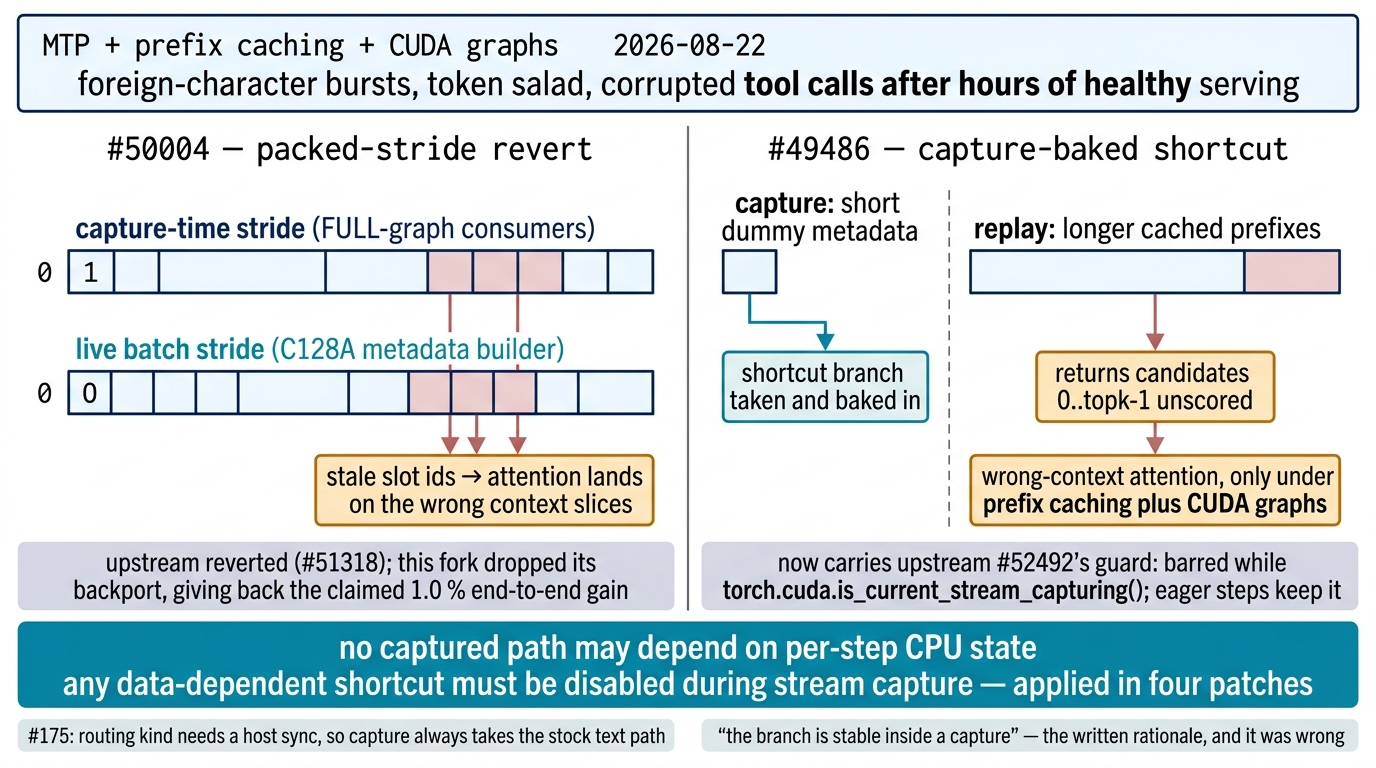
\includegraphics[width=\textwidth]{figures/ch07-capture-vs-runtime.png}
\caption{Both of 2026-08-22's silent-corruption incidents share one mechanism:
a decision made at capture time replayed against run-time state that had
drifted. Left: the adaptive top-$k$ backport (\ghissue{50004}) had the C128A
metadata builder write packed rows at the live batch's stride while FULL-graph
consumers retain the capture-time stride, so every row beyond the first read
stale slot ids --- upstream reverted it (\ghissue{51318}) and this fork dropped
its backport, giving back the claimed 1.0\,\% gain. Right: the short-context
indexer shortcut (\ghissue{49486}) is baked in by a capture against short dummy
metadata, then replayed against longer cached prefixes, returning candidates
\code{0..topk-1} unscored; the port now carries upstream \ghissue{52492}'s
guard, barring the shortcut while the stream is capturing. The rule, now
applied in four patches: no captured path may branch on per-step state.}
\label{fig:bugs-capture-drift}
\end{figure}

\section{The stochastic stall: issue \ghissue{141}}
\label{sec:bugs-stall}

The capture-time corruptions at least ended with mechanisms in hand. The
museum keeps one case that has not.

\textbf{Symptom.} A stochastic TP=2 engine death: generation silently
truncates mid-response with no terminal \code{finish_reason}, while
\code{/health} keeps returning 200. The missing \code{finish_reason} is the
earliest reliable signal --- an operator watching only health checks sees
nothing.

\textbf{What is actually known.} The failure samples inside FlashInfer's SM120
sparse-MLA paged-attention fallback. The pinned FlashInfer revision routes
calls of at most 64 rows to its standalone DSv4 decode kernel; larger calls go
to the paged/prefill orchestrator implicated in the stalls. On one reporting
pair of machines, splitting verify-decode calls at 64 rows survived
3{,}145{,}728 generated tokens, while a 65-row split failed in the first
comparison round. That is the entire causal evidence base: the second failing
pair has not repeated the A/B, and the live TP/stream mechanism remains
unknown.

\textbf{The retractions.} Issue \ghissue{143} initially blamed an
admission-cap interaction. The repository's own wording is unambiguous: the
\ghissue{143} ``\code{MAX_NUM_SEQS=16} bad / 32 safe'' admission-cap mechanism
is \textbf{RETRACTED} --- ``every cell in that matrix was $n{=}1$; per-burst
failure probability explains the whole table without an admission-cap
effect.'' The 2026-08-27 changelog records the same demotion (a single-run
hypothesis invalidated by repeated \ghissue{141} bursts), along with the
earlier framing of \code{MAX_NUM_SEQS=32} as a ``safety''
configuration. The docs now state that no tested \code{MAX_NUM_SEQS} is
generally safe and that configuration changes may alter \emph{incidence}
rather than fix the stall --- admission tuning is performance data, not a
safety recommendation.

\textbf{The workaround --- explicitly not a fix.} The default-off patcher
never makes a call larger than 64 rows (gate
\envvar{DSPARK_ENABLE_ISSUE141_SPARSE_MLA_CHUNK}): bigger calls become sequential disjoint 64-row slice views of
the same six row-coupled tensors, sharing caches, workspace, and output
allocation by identity. The fixed 64 is the pinned kernel-dispatch boundary,
not a deployment concurrency threshold. The patcher source-locks not only the
method it rewrites but also the FlashInfer fragments in a \emph{different
package} whose behavior justifies the constant. The docs enumerate the
still-open validation gates (SM121a numerical tests, a two-rank boot proof,
repeated stochastic soaks) and close with the doctrine this chapter keeps
returning to: one clean burst cannot close a stochastic issue.

\begin{hblesson}
For a stochastic failure, keep three columns: observed (a 64/65-row boundary
on one pair), inferred (path avoidance helps), and unknown (the mechanism,
and whether the second pair reproduces the boundary). Labeling the mitigation
``workaround, not root-cause fix'' in the patch itself, and retracting the
earlier hypothesis in the changelog, is the difference between a field guide
and folklore.
\end{hblesson}

\section{Infrastructure: caches, watchdogs, and spin-waits}
\label{sec:bugs-infra}

The \ghissue{141} stall is not the only way this deployment has lost a TP=2
pair mid-serve. The older way was mundane and --- unlike the stall --- was
chased to a complete root-cause chain. The three exhibits here share a
theme: work deferred until first use --- a kernel not yet compiled, a cache
not yet warm, a sleep path never taken --- costs nothing at boot and
everything under load.

\subsection{Issue \ghissue{117}: the JIT-cache death chain}

\textbf{Symptom.} Mid-serve, an entire TP=2 pair would die: one rank stalls,
the peer waits, and after ${\sim}$600 seconds torch's ProcessGroupNCCL
watchdog terminates the group. Post-mortems found zero collective-level
evidence --- the stalled rank logs nothing.

\textbf{Root cause.} A chain: the in-image Triton cache
(\repofile{~/.triton/cache}) lives in the container's writable layer and dies
on every container recreate; the next boot therefore re-JIT-compiles
already-known kernel shapes \emph{mid-serve} the first time traffic hits them;
a rank stalled in compilation leaves its TP peer parked in a collective; and
the 600-second watchdog --- a deadline that
\envvar{VLLM_EXECUTE_MODEL_TIMEOUT_SECONDS} does not extend --- kills the pair.
The field incident recorded exactly this chain from
\code{_prepare_dflash_inputs_kernel} (\Cref{fig:bugs-jit-chain}).

\textbf{Fixes, layered.}
\begin{enumerate}
  \item \emph{Persist the caches.} \envvar{TRITON_CACHE_DIR} moved onto the
    HF volume, mirroring the earlier \envvar{TILELANG_CACHE_DIR} fix from
    issue \ghissue{65}. A third cache was found later, when a validated boot
    still logged mid-serve CuTeDSL compilation --- the B12X MoE backend's
    own compile cache, now pinned via \envvar{B12X_CUTE_COMPILE_CACHE_DIR}.
    Caches that die with containers are a slow-burning fuse: everything
    works until the first recreate under load.
  \item \emph{Warm the shapes.} A post-ready boot sweep materializes the
    enumerable compile-key buckets before real traffic. It was later hardened
    into a deterministic bucket ladder of exact-token prompts mapped through
    the kernel's own \code{next_pow2} block-size formula onto all six live
    cache keys, after review showed the original concurrency-based arms
    could not reach the low buckets at all.
  \item \emph{Bound the damage.} The \ghissue{45224} backport caps an idle
    SHM ring-buffer reader's wait at 5{,}000\,ms so a missed notify
    self-recovers, and releases the reader slot in \code{finally} when a
    consumer raises.
  \item \emph{Instrument the next one.} The PyTorch flight recorder is
    pinned on, with dumps persisted to the HF volume and a named-pipe
    trigger, so a future frozen-but-not-timed-out pair can be poked for
    per-rank collective traces before restart (archive both ranks' dumps
    together --- the files truncate on every dump).
\end{enumerate}

\begin{figure}[htbp]
\centering
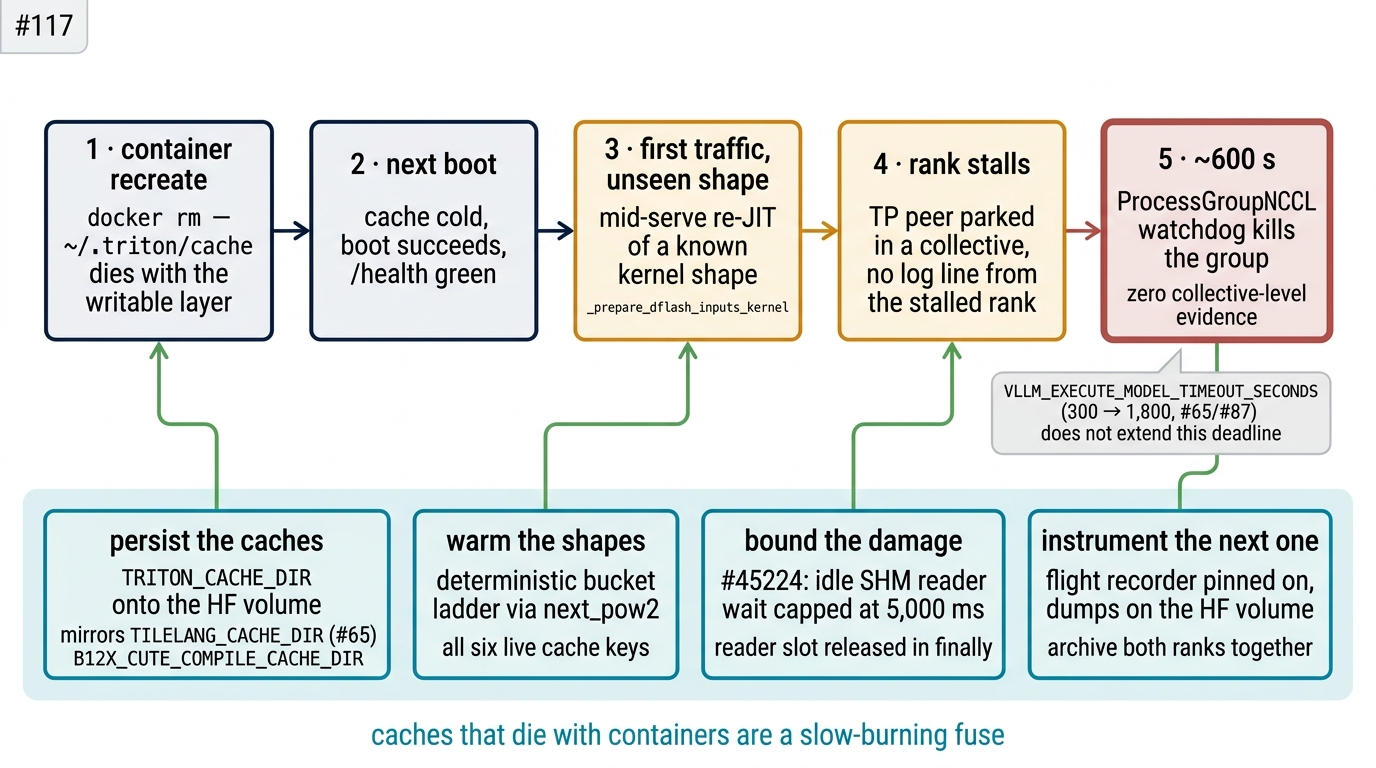
\includegraphics[width=\textwidth]{figures/ch07-jit-death-chain.png}
\caption{Issue \ghissue{117}'s chain. The in-image Triton cache lives in the
container's writable layer and dies on every recreate, so the next boot
re-JIT-compiles already-known kernel shapes mid-serve the first time traffic
reaches them --- the field incident was recorded from
\code{_prepare_dflash_inputs_kernel}. A rank stalled in compilation parks its
TP peer in a collective, and after roughly 600 seconds torch's
ProcessGroupNCCL watchdog kills the pair, leaving no collective-level
evidence; \envvar{VLLM_EXECUTE_MODEL_TIMEOUT_SECONDS} does not extend that
deadline. The four fixes each cut a different link: persist the caches, warm
the six enumerable compile keys at boot, bound the idle reader's wait at
5{,}000\,ms, and wire the flight recorder for the next one.}
\label{fig:bugs-jit-chain}
\end{figure}

\subsection{Issue \ghissue{133}: the compile-key explosion}

A subtler JIT hazard: mixed prefill slices two tensors at the same
traffic-dependent token offset, so Triton's automatic pointer-alignment
specialization produced three cache-key states for the global-top-k kernel.
Crossed with two effective block sizes, that meant six persistent-cache
entries --- and mid-serve compilation stalls whenever traffic found a new
combination. Both
pointers are scalar loads, so alignment specialization bought nothing. The fix
disables alignment specialization for exactly those two pointers and promotes
the stable strides and sizes to \code{tl.constexpr}, collapsing the family to
two deterministic variants, both compiled at boot. The class: a JIT compiler's
\emph{implicit} specialization axes (alignment, dtype, contiguity) multiply
against traffic patterns; enumerate them or they will enumerate themselves in
production.

\subsection{Issues \ghissue{79}, \ghissue{65}, and \ghissue{87}: the small stuff that compounds}

vLLM's cross-process IPC wait spun on \code{busy_loop_s = 1} before sleeping.
Under decode the message gap is always shorter, so the sleep path never
engaged and three to four Grace P-cores spun at max clock, stealing SoC power
budget from the GPU --- fixed by one value, 1\,s $\rightarrow$ 2\,ms
(\ghissue{79}). And \envvar{VLLM_EXECUTE_MODEL_TIMEOUT_SECONDS} was raised
from the stock 300 to 1{,}800 so a legitimate mid-serve TileLang/CuTeDSL JIT
does not get the engine killed while it compiles (\ghissue{65}/\ghissue{87})
--- a stopgap the persisted caches and warmup sweep then made mostly moot.

\section{Vision-Exp integration bugs}
\label{sec:bugs-vision}

The poisoned-transcript dynamic of \Cref{sec:bugs-toolcalls} returns for the
museum's final wing --- the same replay dynamic, in a new subsystem.
Grafting a vision tower onto a text-only serving stack produced its own bug
family --- almost entirely in \emph{validation and identity} logic, not in the
neural network.

\subsection{The image-tag false-positive saga: \ghissue{165}, \ghissue{167}, \ghissue{178}, \ghissue{181}}

The official rule is that images belong in \code{user} messages only;
\code{system}/\code{assistant} images are HTTP 400. The first implementation
scanned message \emph{text} for image markers --- and then spent four
iterations discovering all the ways legitimate text mentions images
(\Cref{tab:bugs-vision-400}). The compounding hazard is that a 400 does not
just fail one request: the offending message stays in the client's history,
so every subsequent request in that session fails too --- the same
poisoned-transcript dynamic as issue \ghissue{55}.

\begin{table}[htbp]
\centering\small
\caption{Four iterations of the Vision-Exp role-validation scan.
\ghissue{165}, \ghissue{167} and \ghissue{181} each narrowed what counts as
``an image'' in non-user roles, while \ghissue{178} instead documented a case
that stays 400 by design; \ghissue{181} closed the self-inflicted loop where
the server's own reply poisoned the session on replay.}
\label{tab:bugs-vision-400}
\begin{tabular}{l>{\raggedright\arraybackslash}p{0.34\textwidth}>{\raggedright\arraybackslash}p{0.42\textwidth}}
\toprule
Issue & False positive & Rule after the fix \\
\midrule
\ghissue{165} & agent system prompts \emph{mentioning} \code{<image>} &
only a paired \code{<image>...</image>} reference or a structured image part
counts \\
\ghissue{167} & a tool result containing \code{cat}/\code{grep} output of the
hotfix itself & \code{tool}/\code{function} \emph{text} is opaque --- never
scanned \\
\ghissue{178} & structured \code{image_url} on a \code{tool} turn &
stays 400 by design (documented): vision-tool results must be replayed on a
\code{user} turn \\
\ghissue{181} & an \emph{assistant reply} that documented the tag, replayed as
history & outside \code{user}, only a structured image part or the raw
placeholder token is an image \\
\bottomrule
\end{tabular}
\end{table}

\subsection{Issue \ghissue{172}: cache identity misses a positional input}

The scan saga was self-inflicted validation logic; the wing's other two
exhibits live deeper, in cache identity and expert routing.

\textbf{Symptom.} An image whose ViT patch grid came out 40$\times$19
intermittently killed EngineCore: 124 embeddings merged into 125 placeholder
slots.

\textbf{Root cause.} The image block's token count is
$122 + \mathrm{compress\_pad}$, and the pad depends on
$\mathrm{start\_pos} \bmod 4$ --- the block layout is a function of \emph{where
in the prompt the image lands}. vLLM's encoder cache hashed image \emph{bytes}
only, so the same photo at a shifted offset reused a block built for a
different pad. The fix salts the multimodal hash with the computed
\code{num_tokens}, and \code{embed_input_ids} now rejects a count mismatch
loudly instead of performing a strict index-put --- a permanent tripwire
against future cache-identity bugs.

\subsection{Issue \ghissue{175}: image tokens routed with text bias}

\textbf{Symptom.} Degraded image understanding with no crash at all.

\textbf{Root cause.} Vision-Exp ships a separate MoE routing bias
(\code{e_score_correction_bias_vl}) for image rows, and it was loaded on every
layer --- but \code{fused_topk_bias} always scored with the \emph{text} bias
plus the \code{tid2eid} hash table. The image placeholder id 129264 is
in-vocab, so the hash-routed layers 0--2 collapsed \emph{every image token}
onto \code{tid2eid[129264]}: one expert assignment for all image content. The
fix routes image rows with \code{bias_vl} and no hash table, leaves text rows
untouched, splits mixed batches --- and, applying the capture rule from
\Cref{sec:bugs-cudagraph}, lets CUDA-graph capture always take the stock text
path (resolving a routing kind needs a host sync, forbidden inside capture).

\section{Synthesis: the recurring failure classes}
\label{sec:bugs-synthesis}

Stripped of their local details, the museum's exhibits sort into six classes
an inference engineer should carry to any stack.

\textbf{Defined-but-unenforced configuration.} \code{max_num_partial_prefills}
existed, defaulted, and was documented --- and the scheduler never read it
(\ghissue{27}). The dead \code{tool_choice} branch guarded by an
enum-to-string comparison is the same class in miniature (\ghissue{55}). Trust
behavior, not schemas; prove a knob's mechanism before A/B-ing its values
(\ghissue{211}).

\textbf{Batch-row versus request identity.} The DSpark draft's persistent KV
was indexed by batch-row position, which vLLM condenses as requests finish, so
one request inherited another's draft state under concurrency (the
Patch~1 slot-map fix of \Cref{ch:specdecode}). The encoder cache keyed by image
bytes while the layout depended on prompt position is the same confusion
(\ghissue{172}). Any state that outlives one step must be keyed by a stable
request-scoped identity, never by position in a mutable batch.

\textbf{Capture-time versus run-time state.} Both silent-corruption incidents
(\ghissue{50004}, \ghissue{49486}), plus the guards independently added in
three other patches, reduce to one rule: a captured graph replays its
capture-time decisions, so no captured path may branch on per-step state.

\textbf{Caches that die with containers.} Triton, TileLang, and CuTeDSL
compile caches in the writable layer turned every container recreate into a
delayed-action TP outage (\ghissue{117}); the vendored DeepGEMM that compiles
only from a warm cache is the same fuse with a different detonator. Persist
JIT artifacts, warm the enumerable shapes at boot, and treat mid-serve
compilation as an incident signal.

\textbf{HTTP 400s that poison replayed history.} Truncated tool calls
(\ghissue{55}), double-encoded arguments (\ghissue{21}), and the vision role
scan (\ghissue{165}--\ghissue{181}) all fail \emph{forward}: the bad message
enters the client's transcript and every later request inherits it. Serving
layers must assume their outputs will be replayed verbatim as inputs.

\textbf{Stochastic bugs and $n{=}1$ evidence.} The \ghissue{141} stall, the
retracted \ghissue{143} hypothesis, the invalidated
\code{MAX_NUM_SEQS=32} safety framing, and the flip-flopping prefill cap all
teach the same statistics: one clean run closes nothing, one dirty run blames
nothing, and mitigations must be labeled as such until the mechanism is in
hand.

Almost nothing in this museum announced itself. The scheduler starved decode
lanes with the preemption counter at zero; the hybrid cache re-prefilled
while its hit rate looked healthy, and then reported hits backed by KV that
no longer existed; the drafter read another request's history; two of this
fork's own performance backports corrupted output after hours of clean
serving. Crashes turn out to be the cheap failures here, because they arrive
with a stack trace and a timestamp --- what costs weeks is a system every
counter reports as fine. That is why the ledger habits in these entries
(labeling the workaround, recording the retraction, keeping the ``no rescue
claim'' sentence) are not paperwork around the engineering; on failures with
no signal, the evidence trail \emph{is} the engineering.

\FloatBarrier
\section*{Takeaways}

\begin{itemize}
  \item Prompts must never end in a dead state: any transcript shape a
    client can legally send needs a defined generation header, and encoder
    patches need fail-closed self-checks (\ghissue{52}/\ghissue{120}).
  \item Trust behavior, not schemas: \code{max_num_partial_prefills} was
    defined, defaulted and documented while the scheduler never read it
    (\ghissue{27}), so prove a knob's mechanism before A/B-ing its values
    (\ghissue{211}). Report truncation truthfully, and measure before blaming
    the exotic subsystem --- \ghissue{191}'s ``grammar race'' was reasoning
    outrunning \code{max_tokens}.
  \item A captured graph replays its capture-time decisions, and any state
    that outlives a step must be keyed by a stable request identity rather
    than a batch row: both silent-corruption incidents
    (\ghissue{50004}, \ghissue{49486}), the drafter's ring buffers, and an
    encoder cache keyed by image bytes while the layout depended on prompt
    position (\ghissue{172}) are one rule seen four ways.
  \item Persist every JIT cache, warm every enumerable compile key at boot,
    and wire forensics before the next stochastic TP loss (\ghissue{117},
    \ghissue{133}, \ghissue{141}).
  \item Write the ledger honestly: label workarounds, record retractions,
    keep the ``no rescue claim'' sentences --- future operators debug with
    your evidence, not your optimism.
\end{itemize}

\chaptertransition{One subsystem keeps reappearing in these exhibits, and it
is not a peripheral one. The speculative drafter broke the batch-identity
rule, corrupted itself silently under concurrency, and took three patches to
make correct --- and it is also the only reason this hardware serves at a
usable rate, since on a machine that must stream sixteen-plus gigabytes of
weights per decode step, draft acceptance is the single lever that multiplies
throughput. The next chapter takes DSpark apart on both counts at once,
because the private state that makes the drafter fast is exactly the state
that made it fail. The uncomfortable part is how quietly it failed: nothing
crashed, nothing was logged, and the only witness was a number most operators
never chart.}
